\chapter{Quantum Estimation}
% Section on density operator
In this chapter we identify the anatomy of the metrology problem and formulate it
in the language of quantum channels and statistical inference. Once this is done we obtain a generic recipe to obtain POVM independent
precision bounds.
\section{Statistical Inference}
\subsection{Estimators}
Any experiment one realizes has an underlying probability distribution over some set $\chi$ that representes the
possible outcomes, specified by the laboratory conditions e.g. temperature, pressure, instrumental precision, initial state and
represented by an element in some parameter space $\Theta$; our objective
is to study this unknown distribution from the experimental results, identifying it \textbf{as precisely as possible} i.e. we have a problem of
statistical inference. Below we present the basic structure of the \textbf{local estimation framework} following \cite{cover_elements_2006,paris_quantum_2009}, its essence is the assumption that the
distribution of study is a member of a known parametric family of probability distributions $\{p(x;\theta)\}_{\theta \in \Theta}$ from which we
must identify the particular $\theta$ that corresponds to our experiment via samples. From this is clear that we need a rule
to go from the sample to the parameter space and that its properties will allow us to study precision, this is the notion that the following
definition seeks to capture.

\begin{definition}
  Given a family $\{p_{\theta}(x)\}_{\theta \in \Theta}$ of probability distributions over some set $\chi$, we call an estimator for $\theta$ a
  sample of size $n$ a function $T:\chi^{n} \to \Theta$. Assuming $\Theta \subseteq \mathds{R}$:
  \begin{itemize}
  \item The difference $T - \theta$ is called \textbf{the error} of the estimator, note this is a random variable
  \item The expected value of the error is called \textbf{the bias}, and if it is zero we say the estimator is \textbf{unbiased}.
  \item Let  $X_{1}, ..., X_{n} \sim p_{\theta}$ be i.i.d random variables, $E[(T(X_{1}, ..., X_{n})-\theta)^{2}]$ is called the \textbf{Mean Square Error} (MSE) of the estimator.
  \item An estimator $T_{1}$ is said to \textbf{dominate} another one $T_{2}$ if its MSE is less than or equal for all $\theta \in \Theta$.

  \end{itemize}
\end{definition}

The MSE is the figure of merit that classifies the estimator $T$, and if it is unbiased we can identify it with $\var{T}$ so that
our credence on $T(x_{1}, ... x_{n})$ is codified in it. We give this last statement a concrete operational meaning through
Chebyshev's inequality:

\begin{theorem}
  Let X be a random variable with finite non-zero variance $\sigma^{2}$ and expected value $\mu$. For any real $k$ the probability of the
  difference between $X$ and $\mu$ being greater than $k\sigma$ is \cite{feller1971introduction}:
$$
P(|X-\mu|\geq k\sigma)\leq \frac{1}{k^{2}}
$$
\end{theorem}

The smaller the variance of $T$ the less likely it is for the difference between $T$ and the actual value $\theta$ to be greater than
$\var{T}$.

\subsection{The Fisher Information}
When one characterizes a measurement apparatus for a quantity $X$ a key property is how \textbf{sensible} it is i.e. given two values  of $X$,
$x$ and $x'$, what is the smallest $\Delta X = |x-x'|$ such that it can differentiate between the two. For estimators there is a similar
connection between a notion of sensitivity and its variance, given by the \textbf{Fisher Information} and the \textbf{Cram\'er-Rao bound}
respectevely.

\begin{definition}
  For a parametric family of probability distributions $\{p_{\theta}\}_{\theta \in \Theta}$ we define the \textbf{Fisher Information} (FI)
  as
  \begin{equation}
    F(\theta) = E\left[\left(\frac{\partial}{\partial \theta}\log{p_{\theta}(x)} \right)^{2}\right] = \int dx \hspace{0.1cm} \frac{(\partial_{\theta} p_{\theta}(x))^{2}}{p_{\theta}(x)}
  \end{equation}
\end{definition}


\begin{theorem}
  The MSE of an unbiased estimator $T$ of the parameter $\theta$ is bounded by
  \begin{equation}
    \var{T}\geq \frac{1}{F(\theta)}.
  \end{equation}
  This inequality is called the \textbf{Cram\'e-Rao bound} (CRB).
\end{theorem}

We say an estimator is \textbf{CR-efficient} if it saturates the CRB \cite{cover_elements_2006,wiseman_quantum_2010}. Note that the CR bound
depends on the family of probability distributions and its parametrization at a given point, not on the estimator. The FI \textbf{quantifies the
  amount of information about the parameter contained in the actual probability distribution} by describing the limits on the amount of
creedence we could assign to \textbf{any} estimation of the parameter $\theta$. The question now is whether the CRB is tight i.e. if there
always exists a CR-efficient estimator, the next theorem shows this is the case asymptotycally.

\begin{definition}
  Given a probability distribution $p_{\theta}$ where $\theta$ is a parameter, we define the \textbf{likelihood} of a sample $\{x_{1},...,x_{n}\}$
  as

  \begin{equation*}
    f_{\theta}(x_{1},...,x_{n}) = \prod_{k=1}^{n}p_{\theta}(x_{k}).
  \end{equation*}

  and the \textbf{Maximum Likelihood Estimator} (MLE)  $\hat{\theta}_{ML} : \chi^{n} \to \mathds{R}$ as
  \begin{equation*}
    \hat{\theta}_{ML}(x_{1}, ..., x_{n}) = \underset{\theta}{\text{arg\hspace{0.05cm}max}}\hspace{0.1cm} f_{\theta}(x_{1},...,x_{n})
  \end{equation*}

\end{definition}

essentially the likelihood measures how probable is to find a given sample provided a value of theta, and the MLE proposes as estimation the
value of the parameter for which this sample is most likely.

\begin{theorem}
The MLE saturates the CRB asymptotically \cite{kay1993fundamentals}.
\end{theorem}

\section{Characterization of Quantum Channels}
Let $\varepsilon_{\gamma}$ be a quantum channel with an unknown $\gamma$ we seek to estimate through some measurement, for this we
need to define an input (initial) state $\rho_{0}$ and perform some measurements on the output. The particular way we measure will
correspond to choosing a POVM $\{\Pi_{x}\}$ that describes the statistics of the experiment. More concretly, the outcomes follow the distribution

\begin{equation}
  \wp(x|\gamma) = \Tr{\Pi_{x}\varepsilon_{\gamma}(\rho_{0})}
\end{equation}

and from it we must infer the value of $\gamma$; from this it is clear that what we got at hand
really is a problem about statistical inference, in which the family of distributions is induced by the POVM.
This reasoning shows all the parts of a \textbf{Metrology Protocol}:

\begin{enumerate}
  \item an initial state
  \item a channel with an unknown parameter one wants to estimate, producing output states $\rho_{\gamma} = \varepsilon_{\gamma}(\rho_{0})$

  \item a measurement strategy, whose statistics are described by a POVM
  \item an estimator producing an estimate $\tilde\gamma$.
\end{enumerate}
in figure \ref{fig:metrology_scheme} this is represented.

\begin{figure}[h]
  \centering
  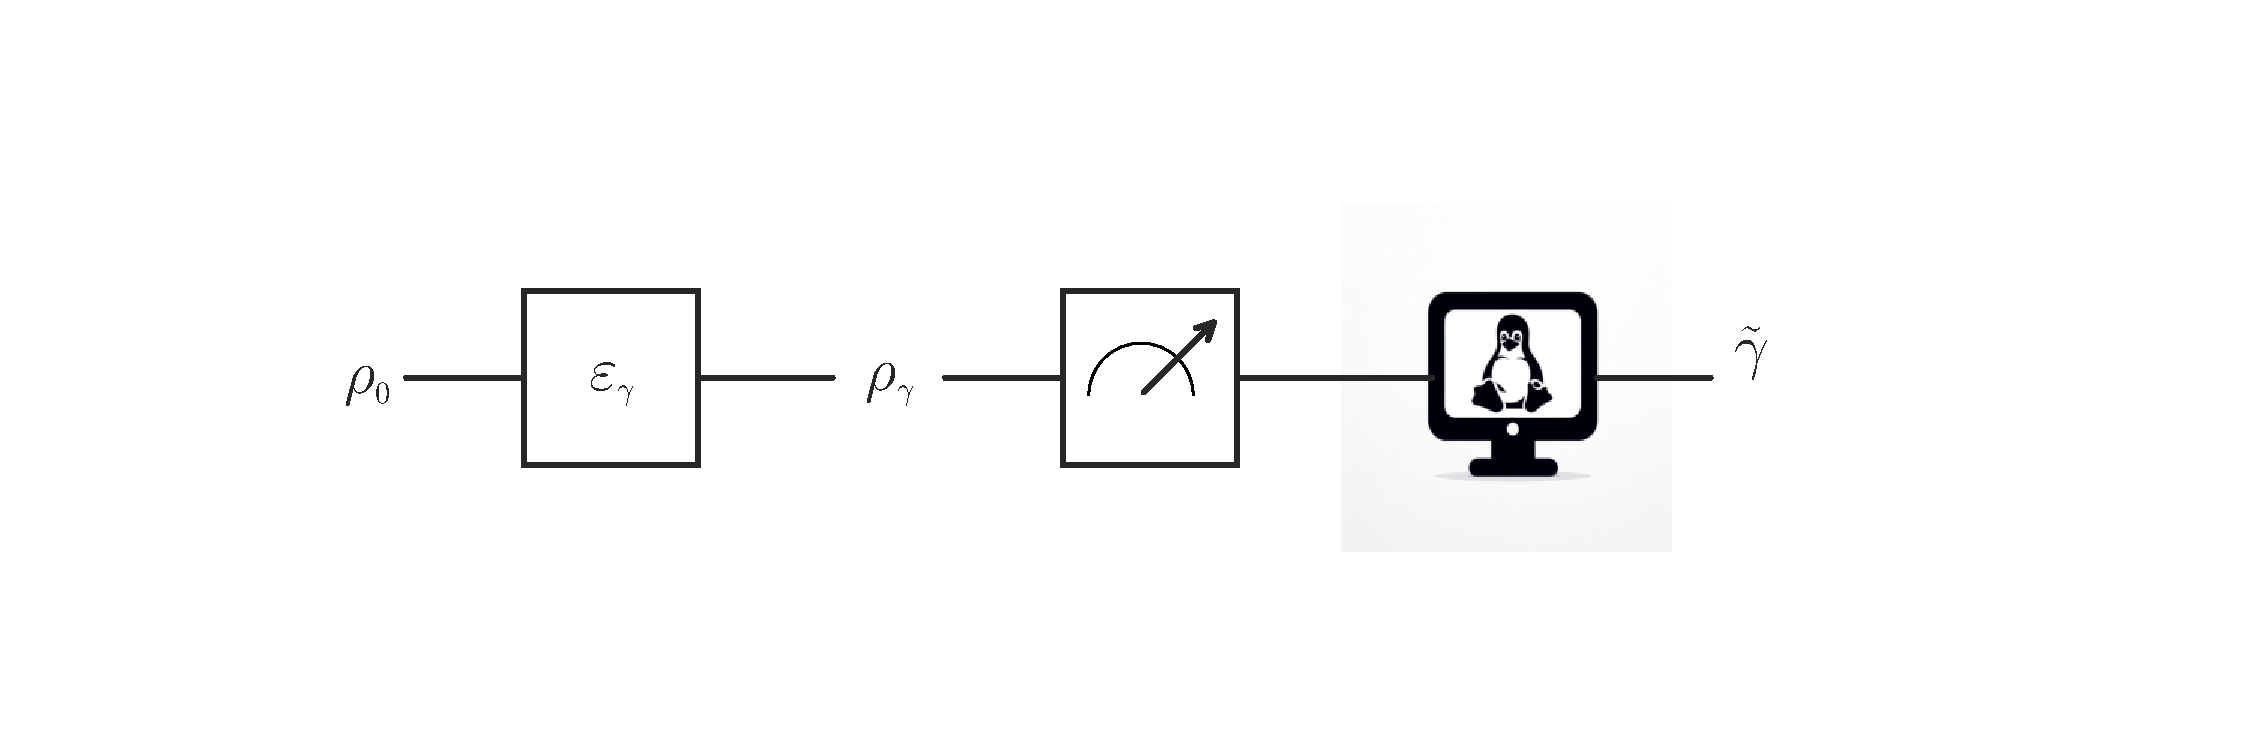
\includegraphics[scale=0.5]{CodeImages/Esquema_Estimacion.pdf}
  \caption{Schematic depiction of a metrology scheme}
  \label{fig:metrology_scheme}
\end{figure}

The objective of quantum metrology is to leverage the nonclassical
aspects of quantum theory to estimate as precisely as possible a
parameter of interest, given a fixed amount of certain
\textbf{resource} involved in the estimation.

\subsection{Optimal POVMs and Precision Bounds}
Different choices of measurement strategy will lead to different
distributions and in turn to different values of FI, this means
that not all the POVMs are made equal. A good
question now is wheter one can bound the FI for all possible
POVMs, this is indeed the case via a procedure proposed in
\cite{braunstein_statistical_1994} to prove theorem \ref{theorem:QFI}.

\begin{theorem}\label{theorem:QFI}
  Let $\varepsilon_{\gamma}$ be a quantum channel parametrized by $\gamma \in \mathds{R}$. For the he Fisher Information of any probability distribution coming from a POVM one has:

  \begin{equation}
F(\gamma) \leq  \Tr{\rho_{\gamma}\Lambda_{\gamma}^{2}}.
\end{equation}

where $\Lambda_{\gamma}$ is a Self-adjoint solution of

\begin{equation}\label{eq:SLD_definition}
  \partial_{\gamma}\rho_{\gamma} = \frac{1}{2}\left(\Lambda_{\gamma}\rho_{\gamma} + \rho_{\gamma}\Lambda_{\gamma} \right).
\end{equation}
and is called the  \textbf{Self-adjoint Logarithmic Derivative} (SLD). Furthermore, there always exists a projective POVM that saturates it \cite{paris_quantum_2009} i.e. there is a maximum FI, called \textbf{Quantum Fisher Information} with value $\Tr{\rho_{\gamma}\Lambda_{\gamma}^{2}}$.
\end{theorem}

\begin{proof}
\begin{align}
  \Tr{\Pi_{x}\partial_{\gamma}\rho_{\gamma}} =& \Re{\Tr{\Pi_{x}\rho_{\gamma}\Lambda_{\gamma}}}\\
   F(\gamma) =& \int dx\hspace{0.1cm} \frac{\Re{\Tr{\Pi_{x}\rho_{\gamma}\Lambda_{\gamma}}}^{2}}{\Tr{\Pi_{x}\rho_{\gamma}}}\\
   F(\gamma) \leq& \int dx\hspace{0.1cm} \frac{|\Tr{\Pi_{x}\rho_{\gamma}\Lambda_{\gamma}}|^{2}}{\Tr{\Pi_{x}\rho_{\gamma}}}\\
   F(\gamma) \leq& \int dx\hspace{0.1cm} \frac{\Tr{\sqrt{\Pi_{x}}\sqrt{\rho_{\gamma}}\sqrt{\rho_{\gamma}}\Lambda_{\gamma}\sqrt{\Pi_{x}}}}{\Tr{\Pi_{x}\rho_{\gamma}}}\\
\end{align}

Using the Cauchy-Schwartz inequality and the normalization of the POVM:

\begin{equation}
F(\gamma) \leq  \Tr{\rho_{\gamma}\Lambda_{\gamma}^{2}}.
\end{equation}

From the spectral decomposition of $\Lambda_{\gamma}$ into rank 1 projectos:
\begin{equation}
\Tr{\partial_{\gamma}\rho_{\gamma}\Lambda} = \sum_{k} \lambda\Tr{(\lambda\rho_{\gamma})\Pi_{k}}
\end{equation}
and noting that:
\begin{align}
\frac{\Tr{\Lambda_{\gamma}\rho_{\gamma}\Pi_{k}}}{\Tr{\rho_{\gamma}\Pi_{k}}} =& \lambda_{k}\\
\Tr{\rho_{\gamma}\Lambda_{\gamma}^{2}} =& \sum_{k} \frac{(\Tr{(\Lambda_{\gamma}\rho_{\gamma})\Pi_{k}})^{2}}{\Tr{\rho_{\gamma}\Pi_{k}}}\\
\Tr{\rho_{\gamma}\Lambda_{\gamma}^{2}} =&\sum_{k} \frac{(\Tr{(\partial_{\gamma}\rho_{\gamma})\Pi_{k}})^{2}}{\Tr{\rho_{\gamma}\Pi_{k}}}
\end{align}
the last line is the FI associated to the POVM formed by the rank 1 projectors of the SLD and so it saturates the inequality.
\end{proof}

This theorem shows there exists POVM independent limits to the variance of parameter estimation
i.e.  \textbf{measurement independent precision bound}. There is no choice of rule for relating outcomes to parameters (estimator) and
measurement strategy (POVM) capable of beating this bound, and so we regard it as a fundamental limit imposed by Quantum Mechanics.
To explore potential quantum advantages use \eqref{eq:SLD_definition} to expand the SLD in the eigenbasis of $\rho_{\gamma}$

\begin{equation}
  \Lambda_{\gamma} = 2\sum_{\substack{nm\\ p_{n}+p_{m}\neq 0}}\frac{\bra{\psi_{n}}\partial_{\gamma}\Lambda_{\gamma}\ket{\psi_{m}}}{p_{n} + p_{m}}\ketbratwo{\psi_{n}}{\psi_{m}}
\end{equation}

where the $p_{k}$'s are the eigenvalues and the $\ket{\psi_{k}}$'s the eigenvectors. Note that the sum is restricted to the support of
$\rho_{\gamma}$ as the SLD is uniquely defined only on it, following \cite{braunstein_statistical_1994} we define it as zero outside it,
this is physically reasonable as the kernel of $\rho_{\gamma}$ plays no meaningful role in the probability distributions induced by the POVMs.
Substituting into the expression for the QFI \cite{paris_quantum_2009}:

\begin{equation}
  \mathcal{F}_{Q}(\gamma) = \sum_{\substack{n\\p_{n}\neq 0}} \frac{(\partial_{\gamma}p_{n})^{2}}{p_{n}} + 2\sum_{\substack{n\neq m\\p_{n} +p_{m}\neq 0}}
  \frac{(p_{m}-p_{n})^{2}}{p_{m}+p_{n}}|\braket{\psi_{n}|\partial_{\gamma}\psi_{m}}|
\end{equation}

The first term is identified as a classical contribution whereas the second one constitutes the quantum addition i.e. there is a quantum
advantage in the optimal probability distribution provided the second term doesn't vanish. This section achieves the basic objective of this
work: stablish the fundamental limits of parameter estimation and identify the possibility for quantum advantages. In the rest we study some particularly important cases, particularly  with phase estimation in this chapter and loss parameters in the next one.

\subsection{Unitary Channels and the Metrological Uncertainty Relations}
Our objective for the rest of this section is to obtain the generic precision bound associated with the QFI of  unitary channels,
this is called the \textbf{Quantum Crame\'er-Rao Bound} (QCRB).
Unitary channels are extremal \cite{watrous2018theory,demkowicz-dobrzanski_elusive_2012} i.e. they
cannot be written as a convex superposition of another channels and have the form:

\begin{equation}
  \varepsilon_{\phi}(\rho)=e^{-iG\phi)}\rho e^{iG\phi}
\end{equation}
where $G\phi$ is a self-adjoint operator that acts as a generator. We begin by studying the effect of state mixing in the QFI, intuitevly one
expects some type of convexity property as mixed states include ignorance additional to the one about the parameter and indeed this is the case \cite{yu2013quantum}, in fact any Fisher Information has this property \cite{cohen1968fisher}. Specifically
this means that for any set of states $\{\rho_1, \dots, \rho_n,\}$
with associated probabilities $\{p_1,\dots, p_n\}$ and for any channel

\begin{equation}
  \mathcal{F}_{Q}[\phi; \sum_{k=1}^{n}\rho_{k}] \leq \sum_{k=1}^{n}p_{k}\mathcal{F}_{Q}[\phi; \rho_{k}].
\end{equation}
Hence to maximize the QFI one must choose a pure initial state.

\begin{theorem}Precision Bound of unitary channels with pure initial state
  For any unitary channel $\varepsilon_{\phi}$ with generator $G$, evolution parameter $\phi$ and a pure initial state $\ket{\psi_{0}}$ one has:
  \begin{align}
    \Lambda_{\phi} =& 2 \partial_{\phi}\rho_{\phi}\\
    \mathcal{F}_{Q}(\phi) =& 4 \Delta G
  \end{align}
  where $\Delta^2G$ is the variance of the generator respect to the
  initial state. Furthermore, the QFI is independent of the value
  of the parameter.
\end{theorem}

\begin{proof}
  As unitary channels preserve the purity we have that for all $\phi$:
  \begin{align}
    \rho_{\phi} =& \rho_{\phi}^{2}\\
    \partial_{\phi}\rho_{\phi}  =& \rho_{\phi}\partial_{\phi}\rho_{\phi} +\partial_{\phi}\rho_{\phi} \rho_{\phi}
  \end{align}
  and so by inspection we get
  \begin{equation}
    \Lambda_{\phi} = 2\partial_{\phi}\rho_{\phi} = -2[ G, \rho ].
  \end{equation}
  For the QFI we do a direct calculation
  \begin{equation}
    \mathcal{F}_{Q}(\phi) = \Tr{\Lambda_{\phi}\partial_{\phi}\rho_{\phi}}= 2\Tr{([G, \rho ])^{2}}
  \end{equation}
\begin{equation}
     ([G, \rho ])^{2}= -e^{-iG\phi}[G, \rho_{0}]^{2}e^{-iG\phi}
\end{equation}
and thanks to the cyclic property of the trace it suffices to calculate the square of the commutator

\begin{align}
\Tr{([G, \rho ])^{2}}=& 2\Tr{G\underbrace{\rho_{0}G\rho_{0}}_{\expectation{\psi_{0}}{G}\ketbra{\psi_{0}}}} - 2\Tr{\rho_{0}G^{2}}\\
  \Tr{([G, \rho ])^{2}}=&-2\expectation{\psi_{0}}{G}\\
  \mathcal{F}_{Q}(\phi) =&  4 \Delta G.
\end{align}
Moments of the generator are always indepedent of the evolution parameter, as can quickly be seen:
\begin{equation}
  \Tr{\rho_{\phi}G^{n}}= \expectation{\psi_{\phi}}{G^{n}}= \expectation{\psi_{0}}{e^{i\phi G}G^{n}e^{-i\phi G}} = \expectation{\psi_{0}}{ G^{n}}
\end{equation}
and hence so is the QFI.
\end{proof}
The previous result gives us the QCRB:

\begin{equation}\label{eq:unitary_QCRB}
  \Delta \phi \Delta G\geq \frac{1}{4}
\end{equation}

and it resembles an uncertainty relation for, but with the
important difference that it is not necessary for $\phi$ to have
an associated observable. An inmediate application of this
result is to the time-energy relation, which can be easily
recovered when $G$ is the hamiltonian of the system
and $\phi$ time; this derivation operationalizes its meaning:
the shorter the time shift the bigger the uncertainty in any
energy measurement, the greatest the uncerainty in the energy the better one could estimate the time shift. The main advantage of this
derivation is that's model independent and does not rely on any type of heuristic, in great contrast to derivations shown in classical
textbooks like \cite{cohen1986quantum,sakurai2020modern}. Similarly one can apply it to the photon number-phase relation that typically
appears in quantum optics \cite{loudon_quantum_2010}, giving an alternative view to the geometric arguments related to the Wigner function.
Note nevertheless that the nature of this \textbf{metrological uncertainty relation} is different from the most general uncertainty relation
derived from operator algebra arguments \cite{gieres2000mathematical}:

\begin{equation}
\Delta A \Delta B \geq \frac{1}{2}|i\braket{A\psi, B\psi} - i\braket{B\psi,A\psi}|
\end{equation}

and they do not coincide for cases like the angular momentum-azimuthal angle case, this is no surprise as our derivation does not rely in
anyway in properties of the adjoint in infinite dimensions and so no inconvenient related to domains happen. To further illustrate this
difference consider the famous position-momentum uncertainty relation: if we choose $G$ to be the momentum $\Delta phi$ is
the estimation uncertainty in a position shift i.e. \eqref{eq:unitary_QCRB} is associated with a particular physical transformation that
can be regarded as a preparation, and if a perfect momentum measurement is performed there will be simultaneously a matter of fact about the
value of the momentum and that of the shift; only momentum measurements are necessary to access the value of the shift.
This is in great contrast to the usual interpretation that comes from the operator derivation in which no preparation is specified, two
measurements are involved, and there is no simultaneous matter of fact. The conclusion we extract from this is that a \textbf{preparation
  parameter} like the shift and a \textbf{physical observable} like the position are fundamentally different quantities, and hence claims
that \eqref{eq:unitary_QCRB} recovers the usual uncertainty relations such as those in \cite{wiseman_quantum_2010} must be taken with care for
they ignore this important subtlety.

\section{Phase Estimation}
The problem of phase estimation consists in determining the phase shift $\theta$ in a channel of the form:
\begin{equation}
  \varepsilon_{\theta}(\rho) = e^{-i\theta G}\varepsilon_{0}(\rho)e^{i\theta G},
\end{equation}

which in general is not unitary as $\varepsilon_{0}$ might include $\theta$ independent non-unitary effects. We choose as
as our system to study the role of environmental effects in precision bounds the case of a photonic system i.e. a \textbf{Bosonic Channel},
under markovian noise.
\subsection{Quantum Advantage in the Unitary Case}
In particular choosing $G=a^{\dagger}a$ as would be the case for example in a Mach-Zender interferometer (MZI) in which $\theta$ is associated
with a phase shift due to the arm-length difference, and taking as input a coherent state $\ket{\psi_{0}}=\ket{\alpha}$ one finds

\begin{equation}\label{eq:shot_noise}
\Delta \theta \geq \frac{1}{4\Delta N}=\frac{1}{\sqrt{N}}
\end{equation}

where $N$ is the average photon number of the input and we have used the poissonian statistics of photon counting for coherent states. The
higher the photon number, the higher precision one can achieve and thus to
increase our knowledge of $\theta$ what must be done is to increase $N$; in this sense we say the photon number acts as a \textbf{resource}.
How much increase in precision one gets from a given increase in $N$ is determined by the characteristics of the initial state, particularly
by how the QFI depends on $N$. It is common terminalogy to call scalings $\Delta \theta \propto N^{-1/2}$ \textbf{shot noise} and  $\Delta \theta \propto N^{-1}$ \textbf{Heisenberg Scaling} \cite{barbieri_optical_2022} \footnote{the origin of these scalings in quantum optics can be tracked down to the dynamics of photodetection, see \cite{wiseman_quantum_2010}}. The really interesting thing about
a particular precision bound is not so much its actual value but the scaling; \eqref{eq:shot_noise} shows that if we identify
classical light as coherent states, then the classical limit of phase estimation in an optical systems is the shot noise.
Then the inmediate question that arises is whether it is possible to surpass it with non-poissonian statistics, embracing the non-classical
aspects of light, for this we consider a squeezed state $\ket{\xi}$ with the same mean photon number, leading to

\begin{equation}
\Delta \theta \geq \frac{1}{N}.
\end{equation}

From here we see that the addition of a non-classical resource, in this quadrature case squeezing, leads to a \textbf{quantum advantage in
  the scaling respect to the mean photon number}. Many other non-classical resources have been shows to lead to advantages in different types
of systems e.g. entanglement, quantum criticality and even quantum chaos \cite{escher_general_2011, giovannetti_quantum_2006, jiao_quantum_2023}.
\subsection{Enviromental effects}
Consider the zero-temperature radiative damping,  restoring the Schr{\"o}dinger picture to regard $\omega $ as a phase shift the channel takes
the form:

\begin{equation}
  \varepsilon_{\omega}(\rho_{0}) = e^{-i\omega t a^{\dagger}a}\left(\sum_{m=0}^{\infty}\frac{(1-e^{-\gamma t})^{m}}{m!}J[e^{-\gamma t a^{\dagger}a/2}a^{m}]\right)e^{i\omega t a^{\dagger}a}.
\end{equation}

For coherent and squeezed state as input one finds respectevly \cite{jiao_quantum_2023}

\begin{equation}
\mathcal{F}_{Q}(\omega) = 4t^{2}e^{-\gamma t}N, \mathcal{F}_{Q}(\omega) \leq \frac{2Nt^{2}}{e^{2\gamma t}-1}
\end{equation}

so not only does the presence of noise degrade the Heisenberg scaling to shot noise but also an exponential decay with time appears even
for small losses, making also harder an experimental implementation as now there exists an optimal \textbf{encoding time}. This exponential
decay of the QFI, proper of markovian models, is sometimes referred to as the \textbf{no-go theorem of Quantum Metrology} although
ways to bend it have been proposed e.g. including environment monitoring, control strategies and non-markovian models
\cite{albarelli_restoring_2018, ,jiao_quantum_2023, liu2017quantum}.

\section{Loss Parameter Estimation in Bosonic Channels}
In this section we follow \cite{adesso_optimal_2009, monras_optimal_2007} to study the problem of loss parameter estimation in a zero
temperature environment (e.g. a leaky QED cavity). These types of channels are governed by the master equation:

\begin{equation}
  \partial_{t} \rho = \gamma(a\rho a^{\dagger} -\frac{1}{2}\{a^{\dagger}a, \rho\})
\end{equation}

where $a,a^{\dagger}$ are the bosonic canonical operators, the objective is to estimate $\gamma$. Notice in first place that this form
is inadequate for the previous formalism as the derivative si taken respect to time instead of $\gamma$, to circumbert this we consider
instead the problem for an adimensional $\tau$:

\begin{equation}
  \partial_{\tau} \rho = a\rho a^{\dagger} -\frac{1}{2}\{a^{\dagger}a, \rho\}
\end{equation}

and later we'll restablish $\gamma$ and $t$ via an appropiate reparametrization, following \cite{adesso_optimal_2009,monras_optimal_2007}.
The form of the channel is the same as in the previous case, with the only difference that here we omit the rotating terms as they are not of
interest:

\begin{equation}
 \varepsilon_{\tau}(\rho_{0}) = \sum_{m=0}^{\infty}\frac{(1-e^{-\tau})^{m}}{m!}J[e^{-\tau a^{\dagger}a/2}a^{m}]\rho_{0}.
\end{equation}
For this case we examine three input states with the same mean photon number: Fock, squeezed and coherent;
their QIFs are presented in the following table and plot.

\begin{center}
      % \resizebox{0.8\columnwidth}{!}{
      \begin{tabular}{c c c c }
        % \toprule
        &\textbf{Coherent} & \textbf{Squeezed}  & \textbf{Fock}   \\
        % \midrule
        % Frequency & $Nt^2$& $t^{2} (\frac{1}{2}N^{2}+5N )$ &  $t^{2}(\frac{N^{2}}{2}+N)$\\
        Loss & $N t^{2}e^{-t\gamma}$ & $ t^{2}N \frac{-2e^{\gamma t} +e^{2\gamma t}+2}{(e^{\gamma t}-1)(2e^{\gamma t}N-2N +e^{2\gamma t})}$ & $t^{2}N \frac{1}{e^{\gamma t}-1}$\\
        % \bottomrule
      \end{tabular}
    % }
      \label{tab:table1}
\end{center}

\begin{figure}[h]
    \centering
    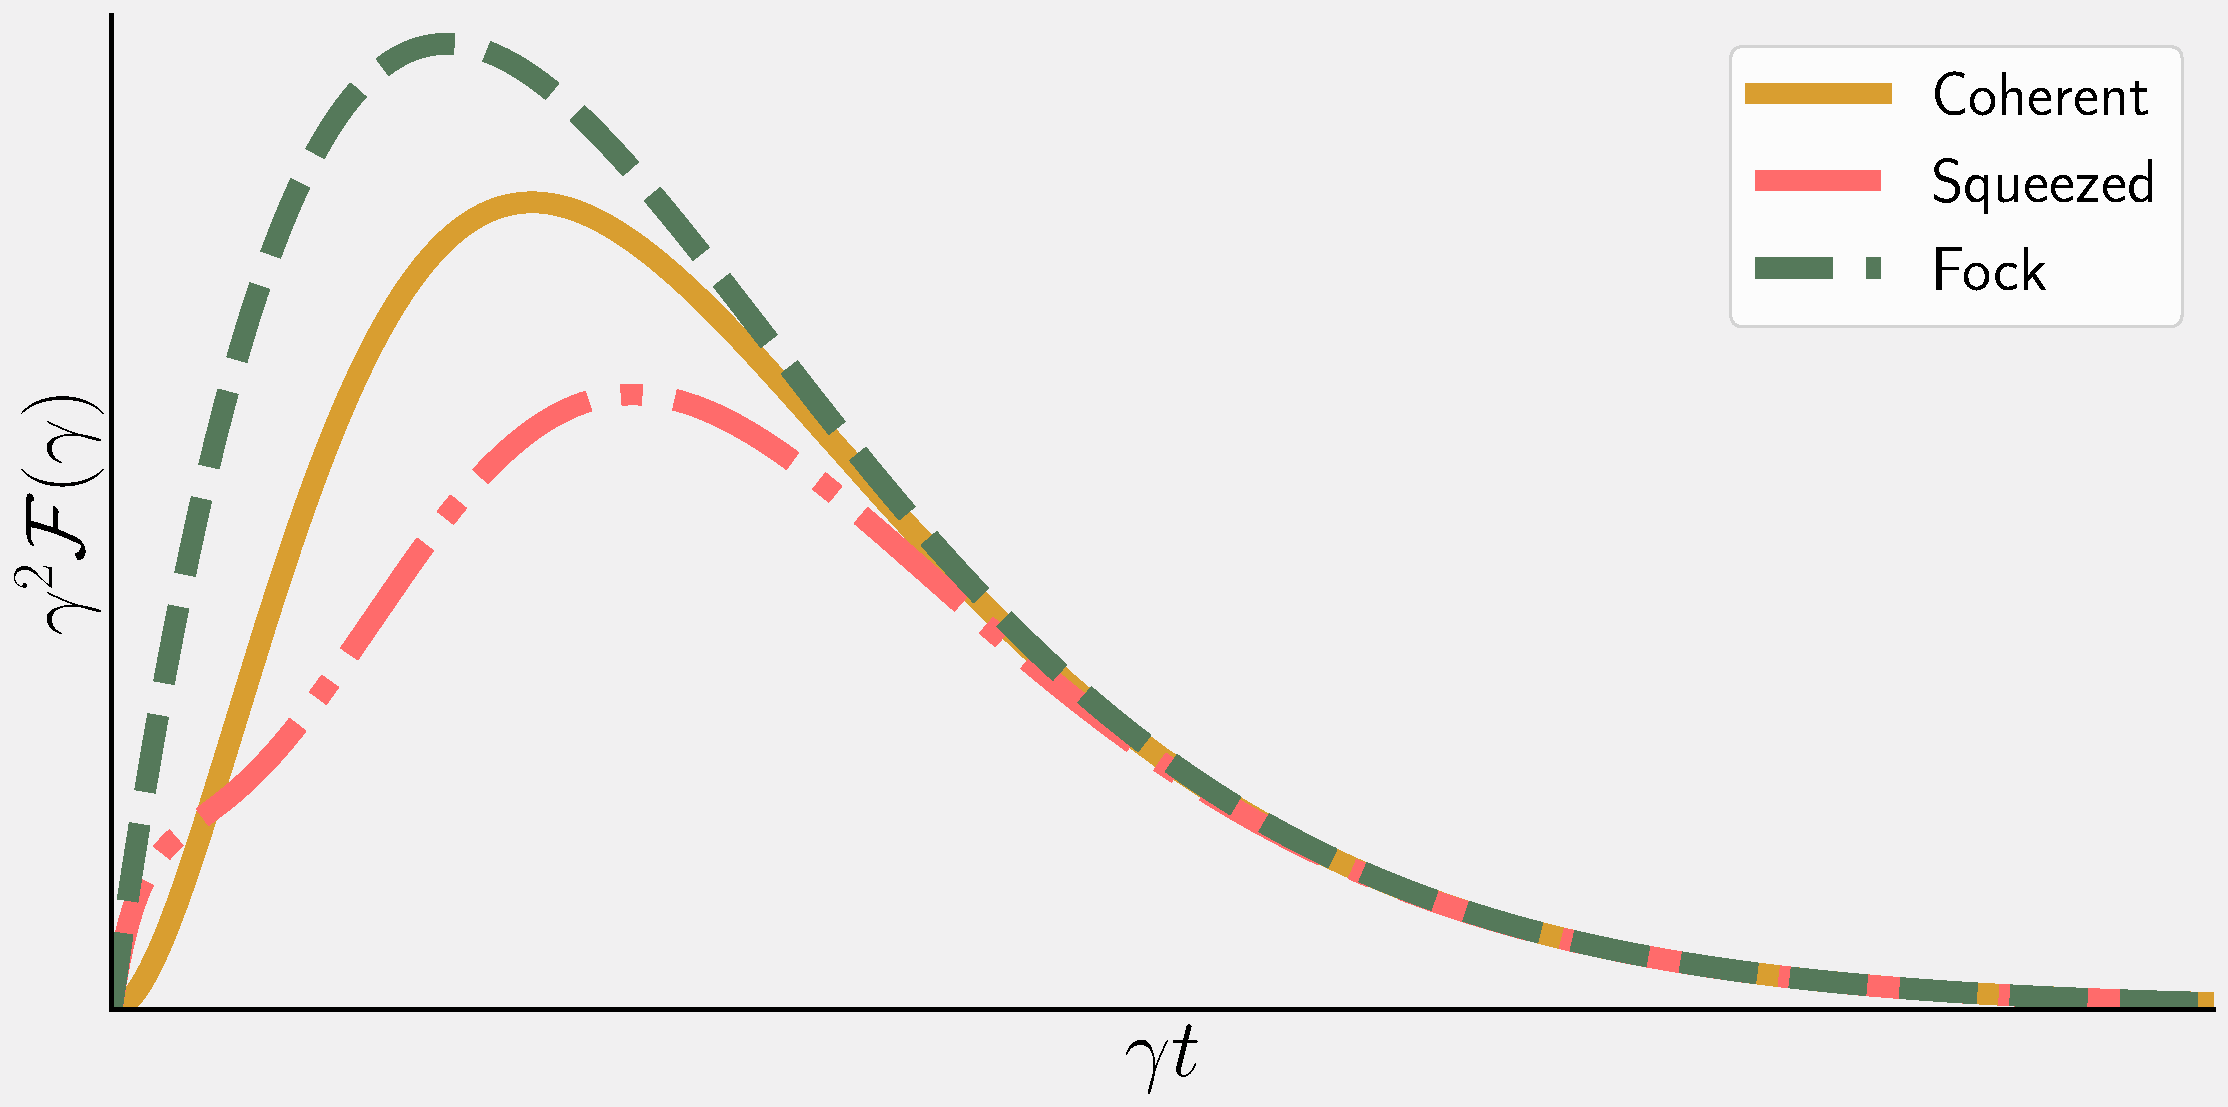
\includegraphics[scale=0.35]{Images/Loss_QFI_Plot.pdf}
    \caption{Adapted from \cite{rossi_2016}}
\end{figure}

Notably, the Fock state is actually the optimal initial state \cite{adesso_optimal_2009} in general and not
only between these 3. Similar to the phase estimation case we see that there exists optimal encoding times and that an exponential decay appears.
